
\chapter{Алгоритмы оценки состояния}
\label{chapter_estimation}

Для реализации обратных связей в контуре управления необходимо обеспечить оценку текущего положения, скорости, кватерниона ориентации и угловой скорости БЛА. Получить данные оценки можно с помощью стандартного набора бортовых датчиков, обычно включающий себя спутниковую систему глобального позиционирования, цифровой барометрический датчик давления, трехосевые электромеханические акселерометр и гироскоп, а также магнитный компас. Однако, в связи с высокими требованиями к массово-габаритным параметрам бортовой системы навигации для небольших летательных аппаратов, страдает качество измерений. Высокий уровень шума побуждает использовать алгоритмы оценки состояния, способные значительно снизить его уровень.

\section{Сигма-точечный фильтр Калмана}

Сигма-точечный фильтр Калмана -- алгоритм оценки состояния, ключевой особенностью которого является отсутствие необходимости линеаризовывать модель \eqref{eq:ekf_system} непрерывной динамической системы. Алгоритм использует модель дискретных измерений.
Задача фильтрации -- найти являющуюся функцией измерений $\bm z_k$ несмещённую оценку вектора состояния системы  $\bm x(t_k)$, минимизирующую дисперсию ошибки  ${\hat{\bm{x}}_k} - \bm x({t_k})$.
Априори оценка вектора состояния $\bm{\hat x}_k^-$ вычисляется как
\begin{equation} \label{eq:ukf_apr}
{\bm{\hat x}}_k^-  = \sum\limits_{i = 0}^{2N} {{w^i} \cdot } \,f\left( {{\bm{X}}_k^i} \right),
\end{equation}
Аргументами функции $f$ в выражении \eqref{eq:ukf_apr} являются так называемые сигма-точки, выбор которых определяется соотношениями
\begin{equation} \label{eq:ukf_points}
\begin{aligned}
&{{\bm{X}}_k^0 = {{\bm{x}}_{k - 1}}},
\\
&{{\bm{X}}_k^i = {{\bm{x}}_{k - 1}} + \sqrt {N + {{\lambda }}}  \cdot {{\left( {\sqrt {{{\bm{P}}_{k - 1}}} } \right)}^i}}, \quad {i = 1,...,N}
\\
&{{\bm{X}}_k^i = {{\bm{x}}_{k - 1}} + \sqrt {N + {{\lambda }}}  \cdot {{\left( {\sqrt {{{\bm{P}}_{k - 1}}} } \right)}^{i - N}}}, \quad {i = N + 1,...,2N}
\end{aligned}
\end{equation}
где
${{{\left( {\sqrt {{{\bm{P}}_{k - 1}}} } \right)}^i}}$
обозначает  $i$-й столбец матрицы ${\sqrt {{{\bm{P}}_{k - 1}}} }$.  Здесь используется разложение Холецкого \cite{Verbjitsky01} вида
${\bm{P}} = \sqrt {\bm{P}} {\sqrt {\bm{P}} ^T},$
где $\sqrt {\bm{P}}$ -- нижняя треугольная матрица. $N$ -- размерность оцениваемого вектора состояния. Весовые коэффициенты в формуле \eqref{eq:ukf_apr} вычисляются как
\begin{equation}
{w^0} = \frac{{{\lambda }}}{{{{\lambda }} + N}},
\quad
{w^i} = \frac{1}{{2\left( {{{\lambda }} + N} \right)}},
\quad
i = 1,...,2N.
\end{equation}
Оценка матрицы ковариации может быть получена по формуле
\begin{equation} \label{eq:ukf_p_apr}
{\bm{P}}_k^ -  = \sum\limits_{i = 0}^{2N} {{w^i}\left( {f\left( {{\bm{X}}_k^i} \right) - {\bm{\hat x}}_k^ - } \right)} {\left( {f\left( {{\bm{X}}_k^i} \right) - {\bm{\hat x}}_k^ - } \right)^{{T}}} + {\bm{Q}},
\end{equation}
где $\bm{Q}$ -- ковариационная матрица шума системы.
При этом весовые коэффициенты в формулах \eqref{eq:ukf_apr} и \eqref{eq:ukf_p_apr} совпадают за исключением коэффициента  ${w^0}$, который в формуле \eqref{eq:ukf_p_apr} принимает значение \cite{Kulikova01}
\begin{equation}
w^0 = \frac{{{\lambda }}}{{{{\lambda }} + N}} + 1 - {{{\alpha }}^2} + {{\beta }},
\end{equation}
где
${{\alpha }} \in \left[ {{{10}^{ - 4}},1} \right]$
-- параметр, определяющий разброс сигма-точек вокруг среднего.
Параметр ${{\beta }}$  позволяет учесть априорные данные о функции плотности вероятности неизвестного вектора состояния системы (для нормального распределения  ${{\beta }} = 2$). Наконец, ${{\lambda }} = 3{{{\alpha }}^2} - N$ -- параметр масштабирования.
Далее происходит коррекция сделанных на предыдущем этапе оценок вектора состояния и матрицы ковариации с помощью вектора и модели измерений.
С помощью функции $h$ из уравнений \eqref{eq:ekf_mes} сигма-точки \eqref{eq:ukf_points} отображаются в пространство измерений, где также делается оценка среднего и матрицы ковариации
\begin{equation}
{\bm{\zeta }}_k^i = h\left( {{\bm{X}}_k^i} \right),
\end{equation}
\begin{equation}
{{{\bm{\hat z}}}_k} = \sum\limits_{i = 0}^{2N} {{w^i} \cdot } \,{\bm{\zeta }}_k^i,
\end{equation}
\begin{equation} \label{eq:ukf_s_k}
{{\bm{S}}_k} = \sum\limits_{i = 0}^{2N} {{w^i}\left( {{\bm{\zeta }}_k^i - {{{\bm{\hat z}}}_k}} \right)} {\left( {{\bm{\zeta }}_k^i - {{{\bm{\hat z}}}_k}} \right)^{{T}}} + {\bm{R}},
\end{equation}
где $\bm R$ -- ковариационная матрица шума измерений. Окончательные оценки для вектора состояния и матрицы ковариации получаются по формулам
\begin{equation}
{\bm{\hat x}}_k^ +  = {\bm{\hat x}}_k^ -  + {{\bm{K}}_k}({{\bm{z}}_k} - {{{\bm{\hat z}}}_k}),
\end{equation}
\begin{equation}
{\bm{P}}_k^ +  = \left( {{\bm{E}} - {{\bm{K}}_k}{{\bm{T}}_k}} \right){\bm{P}}_k^ - ,
\end{equation}
где
\begin{equation}
{{\bm{T}}_k} = \sum\limits_{i = 0}^{2N} {{w^i}\left( {{\bm{X}}_k^i - {\bm{\hat x}}_k^ - } \right)} {\left( {{\bm{\zeta }}_k^i - {{{\bm{\hat z}}}_k}} \right)^{{T}}},
\end{equation}
\begin{equation}
{{\bm{K}}_k} = {{\bm{T}}_k}{\bm{S}}_k^{ - 1}.
\end{equation}

\section{Использование алгоритмов оценки состояния для идентификации параметров БЛА}

Некоторые из динамических свойств объекта измерить достаточно просто, например общую массу или физические размеры квадрокоптера, для измерения других параметров требуется проводить достаточно трудоемкие операции.

Отличной альтернативой является использование расширенного фильтра Калмана, с помощью которого возможно определять или уточнять некоторые параметры динамики квадрокоптера. Например, чтобы оценить аэродинамические константы $k$ и $b$, используем их как составляющие вектора состояния, вместе со скоростью и угловой скоростью:
\begin{equation}
\bm x = (\bm v^I, \bm \Omega^B, k, b)^T.
\end{equation}
При этом в качестве вектора измерений будем использовать
\begin{equation}
\bm z = (\bm v^I, \bm \Omega^B, \dot{\bm v^I}, \dot{\bm \Omega^B})^T.
\end{equation}
Как показывают эксперименты, в результате простого маневра -- взлета и разворота на $\frac{\pi}{2}$, который аппарат сможет выполнить относительно успешно даже с приблизительно известными параметрами, оценка коэффициентов $k$ и $b$
сходится к реальной. Известные параметры модели перечислены в Таблице \ref{tb:observer_params} , графики, демонстрирующие сходимость оценки к реальным значениям на рисунке \ref{fig:observer_k_b}, где красной линией изображена оценка, зеленой -- начальное приблизительное значение, синей -- истинное значение модели.
\begin{figure}[h!]
	\centering
	\subfloat[Оценка аэродинамического коэффициента пропеллера $k$]{%
		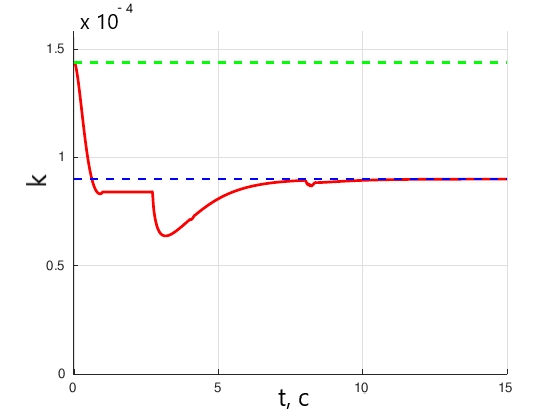
\includegraphics[clip,width=0.44\columnwidth]{k}%
	}
	\quad
	\subfloat[Оценка аэродинамического коэффициента пропеллера $b$]{%
		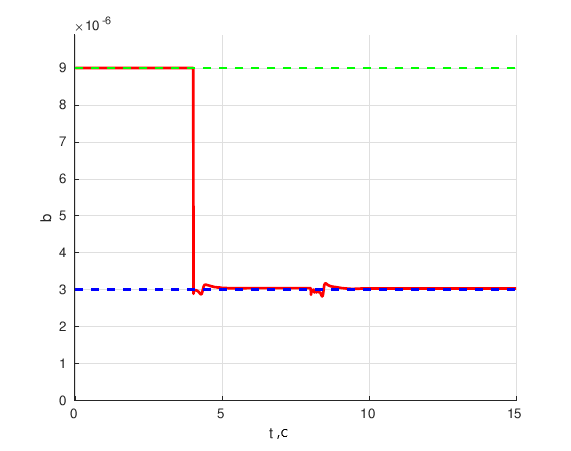
\includegraphics[clip,width=0.44\columnwidth]{b}%
	}
	\caption{ -- Уточнение параметров динамики БЛА}
	\label{fig:observer_k_b}
\end{figure}
